\chead{\textit{Results}}  				
\section{Results}

\subsection{Three Node System}
\label{sec:res:tns}
% TODO Move after mathematical formulations and implementation and then write equations again for this example

The following section describes the \gls{tns} that will be used to further explain the mathematical formulations from section (\ref{sec:math-form}). The system consists of three nodes. At each of them, a different set of generators and storages is located. Each node has a different multi-period demand vector. To simplify the equations and make them easier to understand, only two time steps are considered. The nodes are connected by a total of three transmission lines. Thus, every node has two neighbours. All network elements must meet the requirements described in section (\ref{sec:app:mod-framework}). The network layout is shown in figure (\ref{fig:tns}). One can see that at node one, depicted as N1 in the figure, there are two generators and one storage. At the remaining nodes, only one generator is located. Thus, the system consists of four generators and one storage.

%TODO Make own graphic for three node system
\begin{figure}[h]
	\centering
	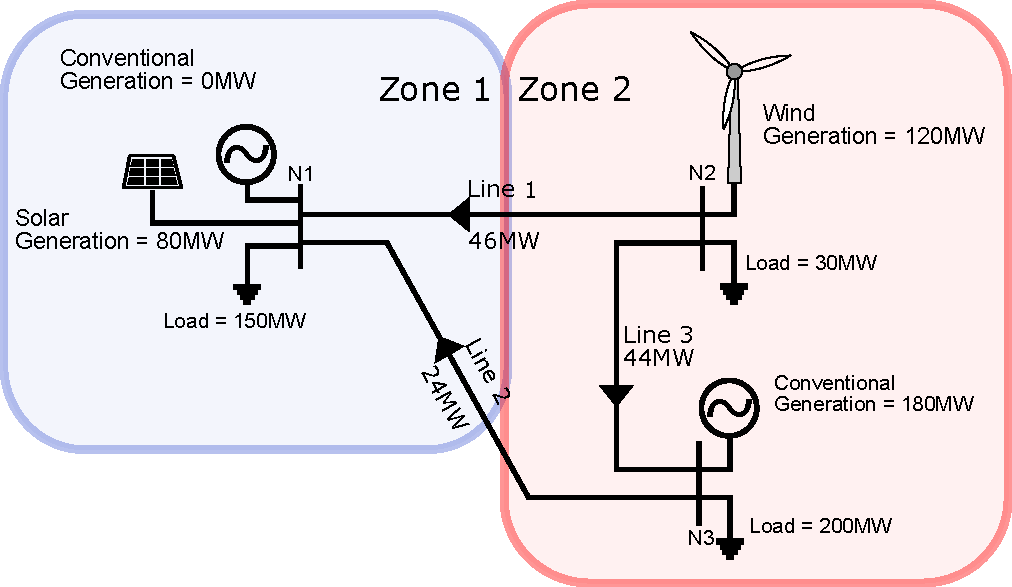
\includegraphics[width=0.8\textwidth]{three-node-system.png}
	\caption{Exemplary Three Node System}
	\label{fig:tns}
\end{figure}

In the following, the equations for the generator and storage subproblem are applied to the \gls{tns}. The aim here is to illustrate the optimization models with a straightforward example so that the reader can more easily follow the rest of the thesis.